\documentclass{article}
\usepackage[utf8]{inputenc}
\bibliographystyle{plain}

\title{Bachelor Thesis}
\author{Jacob Borg }
\date{October 2020}

\usepackage{natbib}
\usepackage{graphicx}
\usepackage{bbding}
\usepackage{enumitem}
\usepackage{tabularx}
\usepackage{multirow}
\usepackage{listings}
\usepackage[colorinlistoftodos,prependcaption,textsize=tiny]{todonotes}

\begin{document}
\maketitle
\thispagestyle{empty}
\clearpage

\tableofcontents
\clearpage

\section{Graphics}
\subsection{Image Caption}
\begin{figure}
    \centering
    \caption{Above caption}
    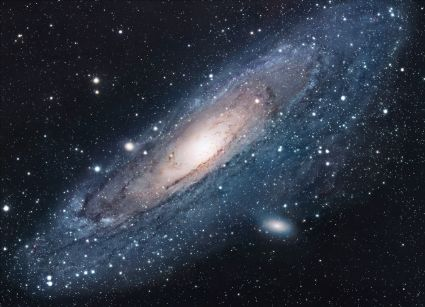
\includegraphics{universe.jpg}
    \label{fig:my_univers}
\end{figure}
\subsection{Images next to each other}
\begin{figure}
    \centering
    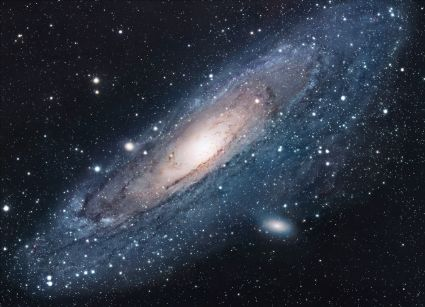
\includegraphics{universe.jpg}
    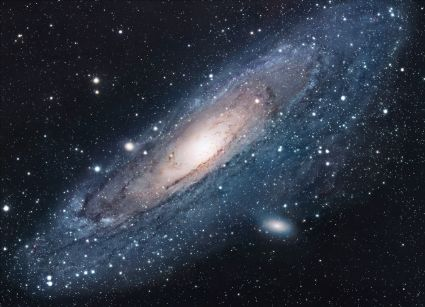
\includegraphics{universe.jpg}
    \caption{Under caption}
    \label{fig:double_universe}
\end{figure}

\section{Reference to image}
reference to my universe \ref{fig:my_univers} \par
\noindent reference to double universe \ref{fig:double_universe}

\section{Reference to page containing the image}
reference to my universe page \pageref{fig:my_univers} \par
\noindent reference to double universe page \pageref{fig:double_universe}

\section{Section, subsection, sub-subsection, paragraph, subparagraph}
\subsection{numbered subsection}
this is subsection
\subsubsection{numbered sub-subsection}
this is sub-subsection
\subsection*{non-numbered subsection}
this is subsection
\subsubsection*{non-numbered sub-subsection}
this is sub-subsection
\paragraph{paragraph}
this is paragraph
\subparagraph{subparagraph}
this is subparagraph

\section{Lists}
\subsection{Bullet list}
\begin{itemize}
    \item pew
    \item pew
\end{itemize}

\subsection{Alternative bullet symbols}
\begin{itemize}
    \item[\Checkmark]  Custom yes
    \item[\XSolidBrush]  Custom no
\end{itemize}

\subsection{Numbered lists}
\begin{enumerate}
    \item one
    \begin{enumerate}[label*=\arabic*.]
        \item one one
    \end{enumerate}
    \item two
\end{enumerate}
\subsubsection{Alternatively numbered lists}
\begin{enumerate}[label*=\Roman*.]
    \item I
    \begin{enumerate}[label*=\roman*.]
        \item I i
    \end{enumerate}
    \item II
    \item III
    \item IV
\end{enumerate}

\section{Table with multiple columns}
\subsection{Various horizontal alignments in columns}
\centering
\begin{tabularx}{0.8\textwidth} { 
  | >{\raggedright\arraybackslash}X 
  | >{\centering\arraybackslash}X 
  | >{\raggedleft\arraybackslash}X | }
 \hline
 AM left & AM center & AM right \\
 \hline
 AM left & AM center & AM right  \\
 \hline
\end{tabularx}
\raggedright

\subsection{Cell spanning multiple columns}
\begin{tabular}{|c|c|}
    \hline
    \multicolumn{2}{|c|}{Am wiiiiiiiiiiiide}\\
    \hline
    smol & smol\\
    \hline
\end{tabular}
\raggedright

\subsection{Vertical alignment in multi-line cells}
\begin{table}[ht]
\centering
\begin{tabular}{cc}
    \hline
    \multirow{2}{*}{Multirow}&X\\
    &X\\
    \hline
\end{tabular}
\label{tab:multiline}
\end{table}
\raggedright

\subsection{Table description and label}

\begin{table}[ht]
\centering
\begin{tabular}{|c|c|}
    \hline
    X & X\\
    \hline
    X & X\\
    \hline
\end{tabular}
\caption{Your caption.}
\end{table}
\raggedright

\subsection{Reference to table}

reference to table \ref{tab:multiline}

\section{Code listing}
\begin{lstlisting}
# Sorts array a[0..n-1] using Bogo sort 
def bogoSort(a): 
    n = len(a) 
    while (is_sorted(a)== False): 
        shuffle(a) 
  
# To check if array is sorted or not 
def is_sorted(a): 
    n = len(a) 
    for i in range(0, n-1): 
        if (a[i] > a[i+1] ): 
            return False
    return True
  
# To generate permuatation of the array 
def shuffle(a): 
    n = len(a) 
    for i in range (0,n): 
        r = random.randint(0,n-1) 
        a[i], a[r] = a[r], a[i] 
\end{lstlisting}
\subsection{With emphasized key words in your favorite programming language}
\begin{lstlisting}[language=Python]
# Sorts array a[0..n-1] using Bogo sort 
def bogoSort(a): 
    n = len(a) 
    while (is_sorted(a)== False): 
        shuffle(a) 
  
# To check if array is sorted or not 
def is_sorted(a): 
    n = len(a) 
    for i in range(0, n-1): 
        if (a[i] > a[i+1] ): 
            return False
    return True
  
# To generate permuatation of the array 
def shuffle(a): 
    n = len(a) 
    for i in range (0,n): 
        r = random.randint(0,n-1) 
        a[i], a[r] = a[r], a[i] 
\end{lstlisting}

\section{Bibliography with book, article and internet link}
\begin{thebibliography}{9}
\bibitem{latexcompanion} 
Michel Goossens, Frank Mittelbach, and Alexander Samarin. 
\textit{The \LaTeX\ Companion}. 
Addison-Wesley, Reading, Massachusetts, 1993.

\bibitem{einstein} 
Albert Einstein. 
\textit{Zur Elektrodynamik bewegter K{\"o}rper}. (German) 
[\textit{On the electrodynamics of moving bodies}]. 
Annalen der Physik, 322(10):891–921, 1905.

\bibitem{knuthwebsite} 
Knuth: Computers and Typesetting,
\\\texttt{http://www-cs-faculty.stanford.edu/\~{}uno/abcde.html}
\end{thebibliography}



\subsection{Todo}
lorem ipsum dolar.
\todo{FIX ME}

\end{document}
